\renewcommand{\SourceFile}{6-geometrie-et-images/src/6-5.ml}

\section[Intersection d'un polygone et d'une fenêtre rectangulaire]{Intersection d'un polygone et d'une\\ fenêtre rectangulaire}

Nous définissons un point de l'écran (que l'on considère muni d'un repère orthonormé direct) comme étant un couple d'entiers $(x,y)$, et un polygone comme étant une suite de finie de points telle que tout couple formé de deux points consécutifs ou du dernier et du premier point de cette suite représente une arête du polygone.
\medskip

Dans tout le problème, les polygones considérés sont par défaut convexes.

\Q
Écrire une fonction OCaml \texttt{clip\_bord} qui, étant donnés un polygone et une droite parallèle à l'axe des abscisses, renvoie l'intersection du polygone avec le demi-plan supérieur à la droite donnée.

\Q
Modifier la fonction précédente pour que l'on puisse choisir une droite qui soit parallèle à l'un ou l'autre des deux axes, et que le demi-plan déterminé par cette droite et utilisé pour l'intersection puisse lui aussi être choisi.

\Q
Écrire une fonction OCaml \texttt{clipping} qui détermine l'intersection d'un polygone avec une fenêtre rectangulaire dont les bords sont parallèles aux deux axes.

\Q
Que se passe-t-il si le polygone considéré n'est pas convexe ? Quelles solutions proposez-vous ?

\Corrige

\Q
On parcourt le polygone et, pour chaque sommet, on regarde si le segment d'extrémités le nouveau sommet et le sommet précédent coupe cette droite ou non. Si oui, on stocke l'intersection dans le polygone intersection, puis on regarde si le sommet courant est dans ou hors de la fenêtre : s'il est dedans, on le place lui aussi dans le polygone de l'intersection.
\medskip

Afin de déterminer l'abscisse $x$ du point d'intersection entre la droite passant par $(x_1,y_1)$ et $(x_2,y_2)$, d'équation $ax+b$ et la droite horizontale d'ordonnée $y$, on résout simplement l'équation $ax+b=y$ où $a=(y_2-y_1)/(x_2-x_1)$. Ce qui donne la formule :
\[
    x = (y-y_1)\frac{(x_2-x_1)}{(y_2-y_1)} + x_1
\]

\begin{center}
\begin{tikzpicture}[scale=1.2]
    \begin{scope}
        \draw (2,0) -- (1,.2) -- (0,1) -- (.4,2) -- (1.7,3) -- (3.1,1.6) -- (2,0);

        \draw[thick] (-.2,.6) -- (3.5,.6);
    \end{scope}

    \draw[-latex, thick] (3.6,1.2) -- (5.2,1.2);

    \begin{scope}[xshift=6cm]
        \draw (0.5, .6) -- (0,1) -- (.4,2) -- (1.7,3) -- (3.1,1.6) -- (2.4125, .6) -- (0.5, .6);
    \end{scope}
\end{tikzpicture}
\end{center}

\lstinputlisting[linerange={1-27}]{\SourceFile}

\Q
La fonction est identique, on ajoute simplement un argument \texttt{t} égal à :\\
0 pour horizontal supérieur\\
1 pour horizontal-inférieur\\
2 pour vertical-droit\\
et 3 pour vertical-gauche.
\medskip

De plus, on utilise une variable \texttt{sg} pour changer le sens des inégalités.
\newpage

\lstinputlisting[linerange={36-63}]{\SourceFile}

\Q
La fonction est très simple : on utilise la fonction \texttt{clip\_bord} pour chaque axe de la fenêtre (représentée par ses coins inférieur gauche et supérieur droit).

\lstinputlisting[linerange={72-78}]{\SourceFile}

Nous remarquons que chaque sommet est visité un nombre fini de fois qui ne dépend pas du nombre de sommets $n$.

\Q
La fonction précédente fonctionne avec des polygones non convexes à la condition que l'intersection se réduise à au plus un polygone. Sinon, les polygones résultant de l'intersection seront réunis par des segments communs aux bords de la fenêtre.

\begin{center}
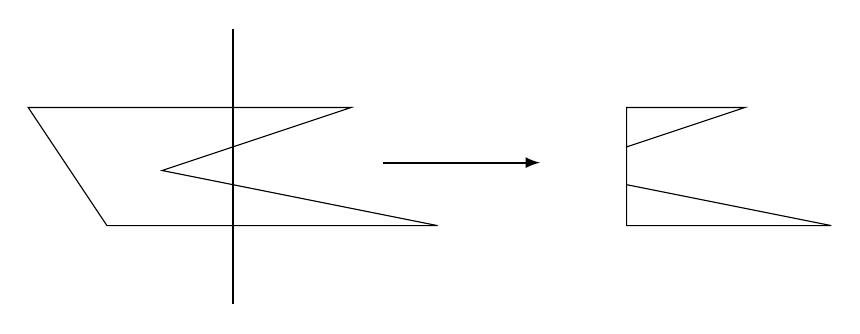
\begin{tikzpicture}
    \begin{scope}
        \draw (1,0) -- (0,1.5) -- (4.1,1.5) -- (1.7,.7) -- (5.2,0) -- (1,0);
        \draw[thick] (2.6,-1) -- (2.6,2.5);
    \end{scope}

    \draw[-latex, thick] (4.5,.8) -- (6.5,.8);

    \begin{scope}[xshift=5cm]
        \draw (2.6,1) -- (4.1,1.5) -- (2.6,1.5) -- (2.6,0) -- (5.2,0) -- (2.6,0.52);
    \end{scope}
\end{tikzpicture}
\end{center}

Une solution est de considérer, lors de la construction de l'intersection avec un demi-plan, les points d'intersection avec la droite frontière et, en partant d'une extrémité, d'associer un polygone à chaque paire. Ceci nous obligerait donc à gérer plusieurs polygones.
\bigskip

\Fin
